\chapter{看涨期权熊市价差}
\section{熊市价差}
在一手看涨期权熊市价差(call bear spread)里,交易者按特定行权价买入一手看涨期权,同时按较低的行权价卖出另一手看涨期权。与牛市价差一样,这也是一个垂直价差。如果标的股票价格下跌,熊市价差一般会盈利。与牛市价差一样,它的潜在盈亏也都有限。不过与牛市价差不一样的是,如果这个价差是用看涨期权来建立的,那熊市价差就是一个收入(credit)价差。\textbf{应当指出,大部分用看涨期权来建立的熊市策略,如果用看期权来建立会更有利。}

有个投资者,他对 XYZ 是看空的,我们可以构建一个熊市价差的示例:XYZ 普通股股票:32,XYZ 10 月 30 看涨期权:3,XYZ 10 月 35 看涨期权:1。

\begin{figure}[h]
    \centering
    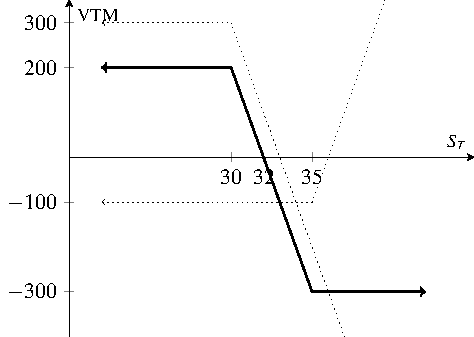
\includegraphics[width=0.7\textwidth]{IMG/Bear spread.pdf}
    \caption{条件:$S_t=32, K_1=30, K_2=35, c_1=3, c_2=1, m=100$}
    \label{fig:bear_spread_using_call_1}
\end{figure}

对熊市价差来说,计算盈亏平衡点、最大潜在盈利和所需投资都相当简单:
\begin{equation}
    \begin{aligned}
        B          & =K_1+c_1-c_2     \\
        max~profit & =c_1-c_2         \\
        max~loss   & =K_1-K_2+c_1-c_2 \\
    \end{aligned}
\end{equation}
\section{熊市价差的选择}
\textbf{一般而言,在标的股票价格更接近较低行权价时建立的熊市价差是最好的熊市价差}。要明白这一点,请注意如果在股票价格等于较高行权价时建立熊市价差会发生什么。此时,价差交易者卖出的看涨期权价值中,大部分是内在价值,只有很少的时间价值(因为它是实值的)。而买入的看涨期权价值中,几乎全是时间价值。这个做法与期权策略家所应该做的刚好相反。期权策略的基本哲学是卖出时间价值,买入内在价值。
\section{后续行动}
策略家必须注意的主要问题是卖出的看涨期权被指派的可能性。如果该价差的空头腿是实值的,没有剩余时间价值,那无论离到期日还有多远,这个价差都应当立刻平仓。导致时间价值消失的原因可能是股票价格显著地高于卖出的看涨期权的行权价,也可能是有股息支付。无论是哪种情况,都应当将这个价差平仓,以避免指派以及由此导致的大笔股票手续费。\textbf{请注意,高收入熊市价差(建立熊市价差时,股票价格远高于较低的行权价)从提前指派的角度来看是非常危险的,因为从一开始卖出的看涨期权的时间价值就很少。}
\section{总结}
看涨期权熊市价差是一种看空(bearish)的策略。这个价差是一个收入价差,要建立这个策略,所需要的只是放弃买入的能力,而不需实际付出现金。因此它是一个还算流行的策略。当有看跌期权存在时,使用看涨期权来建立熊市价差可能不是一个好的选择,应该用看跌期权来建立。
